
%% bare_jrnl.tex
%% V1.4b
%% 2015/08/26
%% by Michael Shell
%% see http://www.michaelshell.org/
%% for current contact information.
%%
%% This is a skeleton file demonstrating the use of IEEEtran.cls
%% (requires IEEEtran.cls version 1.8b or later) with an IEEE
%% journal paper.
%%
%% Support sites:
%% http://www.michaelshell.org/tex/ieeetran/
%% http://www.ctan.org/pkg/ieeetran
%% and
%% http://www.ieee.org/

%%*************************************************************************
%% Legal Notice:
%% This code is offered as-is without any warranty either expressed or
%% implied; without even the implied warranty of MERCHANTABILITY or
%% FITNESS FOR A PARTICULAR PURPOSE! 
%% User assumes all risk.
%% In no event shall the IEEE or any contributor to this code be liable for
%% any damages or losses, including, but not limited to, incidental,
%% consequential, or any other damages, resulting from the use or misuse
%% of any information contained here.
%%
%% All comments are the opinions of their respective authors and are not
%% necessarily endorsed by the IEEE.
%%
%% This work is distributed under the LaTeX Project Public License (LPPL)
%% ( http://www.latex-project.org/ ) version 1.3, and may be freely used,
%% distributed and modified. A copy of the LPPL, version 1.3, is included
%% in the base LaTeX documentation of all distributions of LaTeX released
%% 2003/12/01 or later.
%% Retain all contribution notices and credits.
%% ** Modified files should be clearly indicated as such, including  **
%% ** renaming them and changing author support contact information. **
%%*************************************************************************


% *** Authors should verify (and, if needed, correct) their LaTeX system  ***
% *** with the testflow diagnostic prior to trusting their LaTeX platform ***
% *** with production work. The IEEE's font choices and paper sizes can   ***
% *** trigger bugs that do not appear when using other class files.       ***                          ***
% The testflow support page is at:
% http://www.michaelshell.org/tex/testflow/



\documentclass[journal]{IEEEtran}
%\documentclass[12pt, draftclsnofoot, onecolumn]{IEEEtran}
%
% If IEEEtran.cls has not been installed into the LaTeX system files,
% manually specify the path to it like:
% \documentclass[journal]{../sty/IEEEtran}





% Some very useful LaTeX packages include:
% (uncomment the ones you want to load)


% *** MISC UTILITY PACKAGES ***
%
%\usepackage{ifpdf}
% Heiko Oberdiek's ifpdf.sty is very useful if you need conditional
% compilation based on whether the output is pdf or dvi.
% usage:
% \ifpdf
%   % pdf code
% \else
%   % dvi code
% \fi
% The latest version of ifpdf.sty can be obtained from:
% http://www.ctan.org/pkg/ifpdf
% Also, note that IEEEtran.cls V1.7 and later provides a builtin
% \ifCLASSINFOpdf conditional that works the same way.
% When switching from latex to pdflatex and vice-versa, the compiler may
% have to be run twice to clear warning/error messages.






% *** CITATION PACKAGES ***
%
%\usepackage{cite}
% cite.sty was written by Donald Arseneau
% V1.6 and later of IEEEtran pre-defines the format of the cite.sty package
% \cite{} output to follow that of the IEEE. Loading the cite package will
% result in citation numbers being automatically sorted and properly
% "compressed/ranged". e.g., [1], [9], [2], [7], [5], [6] without using
% cite.sty will become [1], [2], [5]--[7], [9] using cite.sty. cite.sty's
% \cite will automatically add leading space, if needed. Use cite.sty's
% noadjust option (cite.sty V3.8 and later) if you want to turn this off
% such as if a citation ever needs to be enclosed in parenthesis.
% cite.sty is already installed on most LaTeX systems. Be sure and use
% version 5.0 (2009-03-20) and later if using hyperref.sty.
% The latest version can be obtained at:
% http://www.ctan.org/pkg/cite
% The documentation is contained in the cite.sty file itself.






% *** GRAPHICS RELATED PACKAGES ***
%
\ifCLASSINFOpdf
  % \usepackage[pdftex]{graphicx}
  % declare the path(s) where your graphic files are
  % \graphicspath{{../pdf/}{../jpeg/}}
  % and their extensions so you won't have to specify these with
  % every instance of \includegraphics
  % \DeclareGraphicsExtensions{.pdf,.jpeg,.png}
\else
  % or other class option (dvipsone, dvipdf, if not using dvips). graphicx
  % will default to the driver specified in the system graphics.cfg if no
  % driver is specified.
  % \usepackage[dvips]{graphicx}
  % declare the path(s) where your graphic files are
  % \graphicspath{{../eps/}}
  % and their extensions so you won't have to specify these with
  % every instance of \includegraphics
  % \DeclareGraphicsExtensions{.eps}
\fi
% graphicx was written by David Carlisle and Sebastian Rahtz. It is
% required if you want graphics, photos, etc. graphicx.sty is already
% installed on most LaTeX systems. The latest version and documentation
% can be obtained at: 
% http://www.ctan.org/pkg/graphicx
% Another good source of documentation is "Using Imported Graphics in
% LaTeX2e" by Keith Reckdahl which can be found at:
% http://www.ctan.org/pkg/epslatex
%
% latex, and pdflatex in dvi mode, support graphics in encapsulated
% postscript (.eps) format. pdflatex in pdf mode supports graphics
% in .pdf, .jpeg, .png and .mps (metapost) formats. Users should ensure
% that all non-photo figures use a vector format (.eps, .pdf, .mps) and
% not a bitmapped formats (.jpeg, .png). The IEEE frowns on bitmapped formats
% which can result in "jaggedy"/blurry rendering of lines and letters as
% well as large increases in file sizes.
%
% You can find documentation about the pdfTeX application at:
% http://www.tug.org/applications/pdftex





% *** MATH PACKAGES ***
%
%\usepackage{amsmath}
% A popular package from the American Mathematical Society that provides
% many useful and powerful commands for dealing with mathematics.
%
% Note that the amsmath package sets \interdisplaylinepenalty to 10000
% thus preventing page breaks from occurring within multiline equations. Use:
%\interdisplaylinepenalty=2500
% after loading amsmath to restore such page breaks as IEEEtran.cls normally
% does. amsmath.sty is already installed on most LaTeX systems. The latest
% version and documentation can be obtained at:
% http://www.ctan.org/pkg/amsmath





% *** SPECIALIZED LIST PACKAGES ***
%
%\usepackage{algorithmic}
% algorithmic.sty was written by Peter Williams and Rogerio Brito.
% This package provides an algorithmic environment fo describing algorithms.
% You can use the algorithmic environment in-text or within a figure
% environment to provide for a floating algorithm. Do NOT use the algorithm
% floating environment provided by algorithm.sty (by the same authors) or
% algorithm2e.sty (by Christophe Fiorio) as the IEEE does not use dedicated
% algorithm float types and packages that provide these will not provide
% correct IEEE style captions. The latest version and documentation of
% algorithmic.sty can be obtained at:
% http://www.ctan.org/pkg/algorithms
% Also of interest may be the (relatively newer and more customizable)
% algorithmicx.sty package by Szasz Janos:
% http://www.ctan.org/pkg/algorithmicx
\pdfoptionpdfminorversion = 7

\usepackage{amsfonts}
\usepackage{amsmath}
\usepackage{amsthm}
\usepackage{graphicx}
\usepackage{subfigure}
\usepackage{cite}
\usepackage{hyperref}
\hypersetup{
	colorlinks=true,
	linkcolor=black,
	anchorcolor=black,
	citecolor=black}
\usepackage{algorithmic}
\usepackage{algorithm}
\usepackage{courier}
\usepackage{tabularx}



% *** ALIGNMENT PACKAGES ***
%
%\usepackage{array}
% Frank Mittelbach's and David Carlisle's array.sty patches and improves
% the standard LaTeX2e array and tabular environments to provide better
% appearance and additional user controls. As the default LaTeX2e table
% generation code is lacking to the point of almost being broken with
% respect to the quality of the end results, all users are strongly
% advised to use an enhanced (at the very least that provided by array.sty)
% set of table tools. array.sty is already installed on most systems. The
% latest version and documentation can be obtained at:
% http://www.ctan.org/pkg/array


% IEEEtran contains the IEEEeqnarray family of commands that can be used to
% generate multiline equations as well as matrices, tables, etc., of high
% quality.




% *** SUBFIGURE PACKAGES ***
%\ifCLASSOPTIONcompsoc
%  \usepackage[caption=false,font=normalsize,labelfont=sf,textfont=sf]{subfig}
%\else
%  \usepackage[caption=false,font=footnotesize]{subfig}
%\fi
% subfig.sty, written by Steven Douglas Cochran, is the modern replacement
% for subfigure.sty, the latter of which is no longer maintained and is
% incompatible with some LaTeX packages including fixltx2e. However,
% subfig.sty requires and automatically loads Axel Sommerfeldt's caption.sty
% which will override IEEEtran.cls' handling of captions and this will result
% in non-IEEE style figure/table captions. To prevent this problem, be sure
% and invoke subfig.sty's "caption=false" package option (available since
% subfig.sty version 1.3, 2005/06/28) as this is will preserve IEEEtran.cls
% handling of captions.
% Note that the Computer Society format requires a larger sans serif font
% than the serif footnote size font used in traditional IEEE formatting
% and thus the need to invoke different subfig.sty package options depending
% on whether compsoc mode has been enabled.
%
% The latest version and documentation of subfig.sty can be obtained at:
% http://www.ctan.org/pkg/subfig




% *** FLOAT PACKAGES ***
%
%\usepackage{fixltx2e}
% fixltx2e, the successor to the earlier fix2col.sty, was written by
% Frank Mittelbach and David Carlisle. This package corrects a few problems
% in the LaTeX2e kernel, the most notable of which is that in current
% LaTeX2e releases, the ordering of single and double column floats is not
% guaranteed to be preserved. Thus, an unpatched LaTeX2e can allow a
% single column figure to be placed prior to an earlier double column
% figure.
% Be aware that LaTeX2e kernels dated 2015 and later have fixltx2e.sty's
% corrections already built into the system in which case a warning will
% be issued if an attempt is made to load fixltx2e.sty as it is no longer
% needed.
% The latest version and documentation can be found at:
% http://www.ctan.org/pkg/fixltx2e


%\usepackage{stfloats}
% stfloats.sty was written by Sigitas Tolusis. This package gives LaTeX2e
% the ability to do double column floats at the bottom of the page as well
% as the top. (e.g., "\begin{figure*}[!b]" is not normally possible in
% LaTeX2e). It also provides a command:
%\fnbelowfloat
% to enable the placement of footnotes below bottom floats (the standard
% LaTeX2e kernel puts them above bottom floats). This is an invasive package
% which rewrites many portions of the LaTeX2e float routines. It may not work
% with other packages that modify the LaTeX2e float routines. The latest
% version and documentation can be obtained at:
% http://www.ctan.org/pkg/stfloats
% Do not use the stfloats baselinefloat ability as the IEEE does not allow
% \baselineskip to stretch. Authors submitting work to the IEEE should note
% that the IEEE rarely uses double column equations and that authors should try
% to avoid such use. Do not be tempted to use the cuted.sty or midfloat.sty
% packages (also by Sigitas Tolusis) as the IEEE does not format its papers in
% such ways.
% Do not attempt to use stfloats with fixltx2e as they are incompatible.
% Instead, use Morten Hogholm'a dblfloatfix which combines the features
% of both fixltx2e and stfloats:
%
% \usepackage{dblfloatfix}
% The latest version can be found at:
% http://www.ctan.org/pkg/dblfloatfix




%\ifCLASSOPTIONcaptionsoff
%  \usepackage[nomarkers]{endfloat}
% \let\MYoriglatexcaption\caption
% \renewcommand{\caption}[2][\relax]{\MYoriglatexcaption[#2]{#2}}
%\fi
% endfloat.sty was written by James Darrell McCauley, Jeff Goldberg and 
% Axel Sommerfeldt. This package may be useful when used in conjunction with 
% IEEEtran.cls'  captionsoff option. Some IEEE journals/societies require that
% submissions have lists of figures/tables at the end of the paper and that
% figures/tables without any captions are placed on a page by themselves at
% the end of the document. If needed, the draftcls IEEEtran class option or
% \CLASSINPUTbaselinestretch interface can be used to increase the line
% spacing as well. Be sure and use the nomarkers option of endfloat to
% prevent endfloat from "marking" where the figures would have been placed
% in the text. The two hack lines of code above are a slight modification of
% that suggested by in the endfloat docs (section 8.4.1) to ensure that
% the full captions always appear in the list of figures/tables - even if
% the user used the short optional argument of \caption[]{}.
% IEEE papers do not typically make use of \caption[]'s optional argument,
% so this should not be an issue. A similar trick can be used to disable
% captions of packages such as subfig.sty that lack options to turn off
% the subcaptions:
% For subfig.sty:
% \let\MYorigsubfloat\subfloat
% \renewcommand{\subfloat}[2][\relax]{\MYorigsubfloat[]{#2}}
% However, the above trick will not work if both optional arguments of
% the \subfloat command are used. Furthermore, there needs to be a
% description of each subfigure *somewhere* and endfloat does not add
% subfigure captions to its list of figures. Thus, the best approach is to
% avoid the use of subfigure captions (many IEEE journals avoid them anyway)
% and instead reference/explain all the subfigures within the main caption.
% The latest version of endfloat.sty and its documentation can obtained at:
% http://www.ctan.org/pkg/endfloat
%
% The IEEEtran \ifCLASSOPTIONcaptionsoff conditional can also be used
% later in the document, say, to conditionally put the References on a 
% page by themselves.




% *** PDF, URL AND HYPERLINK PACKAGES ***
%
%\usepackage{url}
% url.sty was written by Donald Arseneau. It provides better support for
% handling and breaking URLs. url.sty is already installed on most LaTeX
% systems. The latest version and documentation can be obtained at:
% http://www.ctan.org/pkg/url
% Basically, \url{my_url_here}.




% *** Do not adjust lengths that control margins, column widths, etc. ***
% *** Do not use packages that alter fonts (such as pslatex).         ***
% There should be no need to do such things with IEEEtran.cls V1.6 and later.
% (Unless specifically asked to do so by the journal or conference you plan
% to submit to, of course. )


% correct bad hyphenation here
\hyphenation{op-tical net-works semi-conduc-tor}
\newtheorem{definition}{Definition}
\newtheorem{lemma}{Lemma}
\newtheorem{theorem}{Theorem}
\makeatletter
\newcommand{\removelatexerror}{\let\@latex@error\@gobble}
\makeatother

\begin{document}
%
% paper title
% Titles are generally capitalized except for words such as a, an, and, as,
% at, but, by, for, in, nor, of, on, or, the, to and up, which are usually
% not capitalized unless they are the first or last word of the title.
% Linebreaks \\ can be used within to get better formatting as desired.
% Do not put math or special symbols in the title.
\title{MHCDMC Rouding}
%
%
% author names and IEEE memberships
% note positions of commas and nonbreaking spaces ( ~ ) LaTeX will not break
% a structure at a ~ so this keeps an author's name from being broken across
% two lines.
% use \thanks{} to gain access to the first footnote area
% a separate \thanks must be used for each paragraph as LaTeX2e's \thanks
% was not built to handle multiple paragraphs
%

\author{Qinghui~Zhang,~\IEEEmembership{Student Member,~IEEE,}
	Weidong~Li,~\IEEEmembership{Member,~IEEE,} Qian~Su,~\IEEEmembership{Member,~IEEE}
	and~Xuejie~Zhang,~\IEEEmembership{Member,~IEEE}
	\IEEEcompsocitemizethanks{\IEEEcompsocthanksitem Qinghui Zhang, Qian Su and Xuejie Zhang are with the School of Information Science and Engineering, Yunnan University, Kunming, Yunnan 650091, P.R. China.
		
		E-mail: zhangqinghui@mail.ynu.edu.cn, suqian@ynu.edu.cn,
		xjzhang@ynu.edu.cn
		\IEEEcompsocthanksitem Weidong Li is with the Department of Mathematics, Yunnan University,
		Kunming, Yunnan 650091, P.R. China.
		
		E-mail: weidong@ynu.edu.cn.
	}
	\thanks{(Corresponding author: Xuejie Zhang)}}

% note the % following the last \IEEEmembership and also \thanks - 
% these prevent an unwanted space from occurring between the last author name
% and the end of the author line. i.e., if you had this:
% 
% \author{....lastname \thanks{...} \thanks{...} }
%                     ^------------^------------^----Do not want these spaces!
%
% a space would be appended to the last name and could cause every name on that
% line to be shifted left slightly. This is one of those "LaTeX things". For
% instance, "\textbf{A} \textbf{B}" will typeset as "A B" not "AB". To get
% "AB" then you have to do: "\textbf{A}\textbf{B}"
% \thanks is no different in this regard, so shield the last } of each \thanks
% that ends a line with a % and do not let a space in before the next \thanks.
% Spaces after \IEEEmembership other than the last one are OK (and needed) as
% you are supposed to have spaces between the names. For what it is worth,
% this is a minor point as most people would not even notice if the said evil
% space somehow managed to creep in.



% The paper headers
\markboth{Journal of \LaTeX\ Class Files,~Vol.~14, No.~8, August~2015}%
{Shell \MakeLowercase{\textit{et al.}}: Bare Demo of IEEEtran.cls for IEEE Journals}
% The only time the second header will appear is for the odd numbered pages
% after the title page when using the twoside option.
% 
% *** Note that you probably will NOT want to include the author's ***
% *** name in the headers of peer review papers.                   ***
% You can use \ifCLASSOPTIONpeerreview for conditional compilation here if
% you desire.




% If you want to put a publisher's ID mark on the page you can do it like
% this:
%\IEEEpubid{0000--0000/00\$00.00~\copyright~2015 IEEE}
% Remember, if you use this you must call \IEEEpubidadjcol in the second
% column for its text to clear the IEEEpubid mark.



% use for special paper notices
%\IEEEspecialpapernotice{(Invited Paper)}




% make the title area
\maketitle

% As a general rule, do not put math, special symbols or citations
% in the abstract or keywords.
\begin{abstract}
The abstract goes here.
\end{abstract}

% Note that keywords are not normally used for peerreview papers.
\begin{IEEEkeywords}
high performance computing; resource allocation;
scheduling; approximation algorithm; bag-of-tasks.
\end{IEEEkeywords}






% For peer review papers, you can put extra information on the cover
% page as needed:
% \ifCLASSOPTIONpeerreview
% \begin{center} \bfseries EDICS Category: 3-BBND \end{center}
% \fi
%
% For peerreview papers, this IEEEtran command inserts a page break and
% creates the second title. It will be ignored for other modes.
\IEEEpeerreviewmaketitle


\section{Introduction}
%% 中文测试 Chinese Test

%%由于无人机(unmanned aerial vehicles, UAVs)的可操作性性与不断增长的可负担性,UAV在无线通信系统中有着许多的潜在应用。尤其在一些例如战场或受灾现场等没有通信基础设施覆盖的区域,无人机赋能的移动基站(mobile base stations, MBSs)可以很容易地部署在这些区域并提供无线通信连接。与传统的地面基站相比(base stations, BSs)(包含一些车载基站),为了达到信号覆盖某片区域中位置已知的用户,UAV赋能的MBSs可以部署在任何位置。

% 摘抄自Placement Optimization of UAV-Mounted Mobile Base Stations, Introduction第一段
With their maneuverability and increasing affordability, unmanned aerial vehicles (UAVs) have many potential applications in wireless communication systems [1]. In particular, UAV-mounted mobile base stations (MBSs) can be deployed to provide wireless connectivity in areas without infrastructure coverage such as battlefields or disaster scenes. Unlike terrestrial base stations (BSs), even those mounted on ground vehicles, UAV-mounted MBSs can be deployed in any location and move along any trajectory constrained only by their aeronautical characteristics, in order to cover the ground terminals (GTs) in a given area based on their known locations.

%% 摘抄自“基于多智能体强化学习的大规模灾后用户分布式覆盖优化” 第一段
%在发生重大自然灾害后,地面的基础通信设施通常会遭到毁坏而产生通信中断,重要的通信信息被阻绝,危及受灾群众的生命安全,加剧灾后救援的难度。无人机因为具有快速部署等优点,能够通过装备应急基站提供有效的空地视距链路覆盖受灾地区,在应急通信领域具有广泛的应用前景[1]。
After a major natural disaster, the ground-based communication facilities are usually destroyed and communication is interrupted, and important communication information is blocked, which endangers the lives of the affected people and aggravates the difficulty of post-disaster rescue. UAVs have wide application prospects in the field of emergency communication because of their advantages such as rapid deployment and the ability to provide effective air-ground line-of-sight links to cover the affected areas by equipping emergency base stations [1].

% 原创
%%为了保障人民群众的生命财产安全,加快灾后重建恢复工作,我们需要尽快为用户提供通讯保障。根据实际的通信需求,倚靠人口分布、受灾情况等信息选定一些潜在的可选无人机部署位置。在通信需求的约束下选择最少的无人机数量恢复该片区域的通信网络是一个至关重要的问题。由于大型无人机相对于较小的无人机拥有更大的能源储备,较大的无人机能用更高的功率发射信号,并且能拥有更大的带宽容量来获得更好的信号覆盖性能。因此在本文中我们假设拥有更大信号发射功率的无人机基站,其带宽容量更大。
In order to protect people's life and property and speed up the post-disaster reconstruction and recovery work, we need to provide communication security for users as soon as possible. According to the actual communication demand, some potential optional UAV deployment locations are selected by relying on information such as population distribution and disaster situation. Selecting the minimum number of UAVs to restore the communication network in that area under the constraints of communication needs is a critical issue. Since larger UAVs have larger energy reserves compared to smaller UAVs, larger UAVs can transmit signals with higher power and have greater bandwidth capacity to obtain better signal coverage performance. Therefore, in this paper we assume that the UAV base station with higher signal transmitting power has a larger bandwidth capacity.


% 本文贡献
% 1. 针对无人机基站部署问题中用户需求为实数时,对Bandyapadhyay提出的算法进行了改进,并分析了在无线通信模型中,SINR与功率变化对$\varepsilon$的关系。 
% 2. 我们提出了一种基于重心的分级位置预设算法,对无人机位置进行预设。
% 3. 由于部署无人机的数量及位置是未知的,因此本文对每个用户与无人机之间的SINR进行了预设。经过多次求解,能够很大程度上降低预设值与真实值之间的误差。我们评估了预设SINR与真实SINR之间的差距,以此说明无人机基站部署点位的准确性。

contributions:
\begin{itemize}
	
	\item We improved the algorithm proposed by Bandyapadhyay in \cite{bandyapadhyay_capacitated_2020} when the require of user is real.We also analyze the relationship between SINR and power variation on $\varepsilon$ in the wireless communication model is analyzed.
	
	\item We propose a center-of-gravity-based  hierarchical position presetting algorithm to preset the UAV position.
	
	\item Since the number and location of deployed UAVs are unknown, the SINR between each user and UAV is preset in this paper. After multiple solving, the gap between the preset value and the real value can be reduced significantly. We evaluated the gap between the pre-set SINR and the real SINR as an indication of the accuracy of the UAV base station deployment sites.
\end{itemize}


\section{Related work}
Related work
\section{System model}
\subsection{Network model}
%%%%%% 2022年11月9日23:45:18改
% 版本2(2022年11月9日):在某个可以看做平面的受灾区域中,我们需要为n个位置已知的受灾用户(简称用户)恢复通信服务,用U={u1,...,un}表示用户的集合。用户uj\inU 的位置坐标为loc^u_j(X,Y,0),他请求的通信带宽资源为BR_j。根据受灾用户的分布情况,我们规划了m个无人机可能部署的位置,每个位置上的无人机型号是确定的。为了方便表述,我们用A={a1,...,am}表示这m个可能被部署的无人机的集合。无人机a_i\in A 的位置坐标为loc^a_i(X,Y,h)。Assume that all UAVs fly at the same altitude $h$ such that the coverage range of each UAV is maximized, where $h < R$ and the optimal altitude $h$ can be obtained from the work in \cite{al-hourani_optimal_2014}, e.g., $h = 300$ m. 此外,MBS ai的信号发射功率为pi,且带宽资源有限,为BWi。为了能够尽快为用户恢复通信,在每个无人机带宽资源有限的约束下,我们需要选择部署尽可能少的无人机,并且保证每个用户的通信质量,即用户的信噪比大于一个最小信噪比阈值SINR_min。
%%版本1(2022年10月9日):在某受灾区域中,我们预设了m个位点及可能部署于该位点的MBS。虽然在每个位置部署都MBS能够满足所有用户的通信需求,但这是十分低效且不切实际的。我们需要尽快选择其中尽可能少的位点部署对应的MBS,尽快为n个用户恢复通讯服务。我们分别用U与A表示用户与MBS位点的集合。对于每个用户uj,都有带宽需求BRj。MBS ai的信号发射功率为pi,且带宽资源有限,为BWi。
%对于为了能在保证所有用户的通信信干噪比不小于SINR_min的前提下,尽快为用户恢复通讯,我们需要选择尽可能少的部署MBSs。我们引入决策变量xij与yi。用yi表示是否选择ai作为最终的MBS部署策略,当ai=1表示选择MBS ai。用xij表示是否令ai为uj分配带宽资源提供服务,当xij=1时表明uj被ai服务。
In a disaster area that can be viewed as a plane, we need to restore communication services for $n$ affected users (referred to as users) whose locations are known, and use $U=\left\{u_1,... ,u_n\right\}$ denotes the set of users. The location coordinates of user $u_j\in U$ are $loc^u_j=(X^u_j,Y^u_j,0)$, and the communication bandwidth requirement is $BR_j$. Based on the distribution of affected users, we intend $m$ candidate UAVs deployment. We use $A=\left\{a_1,... ,a_m\right\}$ to denote the set of these $m$ candidate UAVs. The position coordinates of $a_i\in A$ are $loc^a_i=(X^a_i,Y^a_i,h)$, where $h$ is the optimal altitude such that the coverage range of UAV is maximized \cite{al-hourani_optimal_2014}. In addition, all UAVs have the same power $p$ and bandwidth capacity $BW$. In order to be able to quickly restore communication for users, under the constraint of bandwidth capacity per UAV, we need to deploy as few UAVs as possible and guarantee the communication quality for each user, i.e., the user's signal-to-noise ratio (SINR) is greater than a minimum SINR threshold $SINR_{min}$.
% 我们将该问题定义为最小基数信号覆盖问题。
We define the problem as a minimum metric capacitated signal coverage (MMCSC) problem.
%We introduce decision variables $x_{ij}$ and $y_i$. $y_i$ denotes whether to choose $a_i$ as the final MBS deployment policy, and when $y_i=1$ indicates that MBS $a_i$ is chosen. $x_{ij}$ is used to indicate whether to make $a_i$ allocate bandwidth resources for $u_j$ to provide services, and when $x_{ij}=1$ indicates that $u_j$ is served by $a_i$.



% 2022年11月10日
% 
% MMCSC问题中,选择部署A中所有无人机当然能满足所有用户的通信需求,但这无疑是十分浪费资源的与低效的。在单个无人机资源有限的约束下保证服务质量,选择尽可能少的无人机进行部署,能够更快速的进行部署是符合逻辑的。这个问题显然是一个NP-hard问题,因为在【1】中即使没有容量约束的覆盖问题也是NP-hard问题。那么为之设计一个有效的近似算法部署




%%无人机赋能的MBS与用户之间的通信采用sub-6GHz频段的空地对接通信链接,其中视距无线传输(Line of Sight, LoS)占主导地位。a与u之间的路径损耗可以表示为
The communication between the UAV-enabled MBS and the user uses an air-to-ground communication link in the sub-6 GHz band, where Line of Sight (LoS) dominates. A The path loss between $u_j$ and $a_i$ can be expressed as:
\begin{eqnarray}
	\label{eq1}
	{L_{ij}}({\rm{dB}}) = 20\lg ({d_{ij}}) + 20\lg (\frac{{4\pi f}}{c}) + {\eta _{LoS}},
\end{eqnarray}
%其中,d表示a与u之间的距离,f表示载波频率,c代表光速,e代表 LoS 的阴影衰落损耗,是一个常量。a与u之间的信干噪比为
where $d_{ij}$ denotes the distance between $a_i$ and $u_j$, $f$ denotes the carrier frequency, $c$ represents the speed of light, and $\eta _{LoS}$ represents the shadow fading loss of LoS, which is a constant. the signal-to-noise ratio between $a_i$ and $u_j$ is:
\begin{eqnarray}
	\label{eq2}
	SINR_{ij} = \frac{{{G_{ij}}{p}}}{{{N_I} + {N_0}}},
\end{eqnarray}
% G表示a与u之间的信道增益,NI表示该环境中的干扰噪声功率,N0表示白噪声功率。信道增益g受路径损耗影响,满足以下关系
$G_{ij}$ denotes the channel gain between $a_i$ and $u_j$, $N_I$ denotes the interference noise power in this environment, and $N_0$ denotes the white noise power. The channel gain $G_{ij}$ is affected by the path loss and satisfies the following relationship:
\begin{eqnarray}
	\label{eq3}
	{G_{ij}}{p}({\rm{dB}}) = {p}({\rm{dB}}) - {L_{ij}}({\rm{dB}}).
\end{eqnarray}


%注释日期2022年11月10日
%根据以上关系,用户的传输速率可以表示为
%According to the above relationship, $u_j$'s data rate $DR_j$ can be expressed as
%\begin{eqnarray}
%	\label{eq4}
%	D{R_j} = B{R_j}{\log _2}(1 + SIN{R_{ij}}).
%\end{eqnarray}


% 2022年11月10日 
% 根据公式1,2,3,我们可以得到当服务器$a_i\in A$的功率为$p_i$时,最小信噪比为SINR_min时,a_i的服务半径.由于最终选择哪些服务器是未知的,因此干扰噪声N_I也是未知的。我们在此处令N_I=0,我们将在第4节进一步对N_I进行分析。
According to Eq.(\ref{eq1}),(\ref{eq2}),(\ref{eq3}), we can get the coverage radius of $a_i \in A$ when its power is $p$, the minimum SINR is $SINR_{ min} $:
\begin{eqnarray}
	{r_i} = {10^{\left[{{{p}({\text{dB}}) - SIN{R_{\min }}({\text{dB}}) - \eta ({\text{dB}}) - N({\text{dB}})}}\right]/{{20}}}},
\end{eqnarray}
where $\eta({\text{dB}}) = 20 \log{\frac{4\pi f}{c}}({\text{dB}}) + \eta_{LoS}({\text{dB}})$, $N({\text{dB}})=(N_I + N_0)({\text{dB}})$. Since the final selected servers are unknown, the interference noise $N_I$ is also unknown. We hereby set $N_I=0$, and will further study in section 4 $N_I$ for analysis.


% 由公式(4),我们可以把无人机$a_i$

%
Based on the above definition, we can get the integer programming form of the problem.
\begin{align}
	\min \quad  & \sum\nolimits_{{a_i} \in A} {{y_i}}  \label{ip:1}\\
	s.t.\quad &  {x_{ij}} \le {y_i},  \forall {u_j} \in U,\;\forall {a_i} \in A. \tag{\ref{ip:1}{a}}\label{ip:1.1}\\
	&  \sum\nolimits_{{u_j} \in U} {({x_{ij}} \cdot B{R_j})}  \le {y_i} \cdot BW,\forall {a_i} \in A. \tag{\ref{ip:1}{b}}\label{ip:1.2}\\
	&  \sum\nolimits_{{a_i} \in S} {{x_{ij}}}  = 1,\forall {u_j} \in U. \tag{\ref{ip:1}{c}}\label{ip:1.3}\\
	&  {x_{ij}} = 0,\forall {u_j} \in U,\forall {a_i} \in A:SIN{R_{ij}} < SIN{R_{\min }}. \tag{\ref{ip:1}{d}}\label{ip:1.4}\\
	&  {x_{ij}} \in \left\{ {0,1} \right\},\forall u_j \in U,\forall {a_i} \in A \tag{\ref{ip:1}{e}}\label{ip:1.5}\\
	&  {y_{i}} \in \left\{ {0,1} \right\},\forall {a_i} \in A. \tag{\ref{ip:1}{f}}\label{ip:1.6}
\end{align}


%约束(1.1)的含义是,只有选择MBS ai之后,uj才能被ai服务。约束(1.2)是每一个MBS的带宽资源容量资源约束,它服务的用户带宽需求之和不能超过其自身的能力。约束(1.3)的表示每一个用户都必须被服务。约束(1.4)的含义是如果uj被ai服务,那么uj的信噪比要大于SINR_min。约束(1.5)与(1.6)为两个整数决策变量约束。我们将整数规划(1)松弛后能得到其线性规划(2):
Constraint (\ref{ip:1.1}) means that $u_j$ can be served by $a_i$ only after the MBS $a_i$ is selected. Constraint (\ref{ip:1.2}) is the bandwidth resource capacity resource constraint of each MBS, the sum of bandwidth demand of users it serves cannot exceed its own capacity. Constraint (\ref{ip:1.3}) of indicates that every user must be served. Constraint (\ref{ip:1.4}) means that if $u_j$ is served by $a_i$, then the SINR of $u_j$ has to be greater than $SINR_{min}$. Constraints (\ref{ip:1.5}) and (\ref{ip:1.6}) are two integer decision variable constraints. We relax the integer programming(LP) (\ref{ip:1}) to be able to obtain its linear programming (\ref{lp:2}):

\begin{align}
	\min \quad & \sum\nolimits_{{a_i} \in A} {{y_i}}  \label{lp:2}\\
	s.t.\quad &  {x_{ij}} \le {y_i},\forall {u_j} \in U,\forall {a_i} \in A. \tag{\ref{lp:2}{a}}\label{lp:2.1}\\
	&  \sum\nolimits_{{u_j} \in U} {({x_{ij}} \cdot B{R_j})}  \le {y_i} \cdot BW,\forall {a_i} \in A. \tag{\ref{lp:2}{b}}\label{lp:2.2}\\
	&  \sum\nolimits_{{a_i} \in S} {{x_{ij}}}  = 1,\forall {u_j} \in U. \tag{\ref{lp:2}{c}}\label{lp:2.3}\\
	&  {x_{ij}} = 0,\forall {u_j} \in U,\forall {a_i} \in A:SIN{R_{ij}} < SIN{R_{\min }}, \tag{\ref{lp:2}{d}}\label{lp:2.4}\\
	&  {x_{ij}} \ge 0,\forall u_j \in U,\forall {a_i} \in A \tag{\ref{lp:2}{e}}\label{lp:2.5}\\
	&  0 \le {y_i} \le 1,\forall {a_i} \in A. \tag{\ref{lp:2}{f}}\label{lp:2.6}
\end{align}

% 我们能在多项式时间内得到线性规划6的最优解sigma,这个解是一个分数解。在这个解中,对于任意xij>0对应的用户与MBS,它们之间的SINRij>=SINRmin。 在真实的场景中,MBS可以通过频谱复用等方法来增强自身的信号覆盖能力。我们定义SINRmin'(<SINRmin)为采用复用技术之后的最小信干噪比。当SINRmin'<=SINRij<=SINRmin时,ai也可以通过采取复用技术为uj提供具有较好的信号质量的服务。此外,MBS也能通过增加信号功率来增强信号覆盖能力。令pi’为增强之后的功率。
We can obtain the optimal solution $\sigma=(x,y)$ of LP \ref{lp:2} in polynomial time, which is a fractional solution. The cost of the LP solution $\sigma$ (feasible or otherwise), denoted by cost($\sigma$), is defined as $\sum\nolimits_{{a_i} \in A} {{y_i}}$.


In this solution, for any $x_{ij}>0$ , we can ensure that $SINR_{ij}\ge SINR_{\min}$. In a real scenario, MBS can enhance its own signal coverage through spectrum multiplexing and other methods. We define $SINR_{\min}'$($<SINR_{\min}$) as a new minimum SINR after using the multiplexing technique. When $SINR_{min}' \le SINR_{ij} \le SINR_{\min}$, $a_i$ can also provide services with acceptable signal quality for $u_j$ by adopting multiplexing techniques. In addition, MBSs can also increase the signal coverage by enhancing the signal power. Let $p'$ be the power after enhancement.


%对于SINRmin'与pi'这两个变量,他们的变化幅度是有限的。本文并不关注于SINRmin'有多小或pi'有多大,我们只给出了他们变化幅度的定义如下。
For the two variables $SINR_{\min}'$ and $p'$, they have a limited variation. In this paper, we do not focus on how small $SINR_{\min}'$ is or how large $p'$ is; we only give the definition of the magnitude of their variable as follows.
\begin{eqnarray}
	{\varepsilon ^p} = \frac{{{p'} - {p}}}{{{p}}},
\end{eqnarray}


\begin{eqnarray}
	{\varepsilon ^{SINR}} = \frac{{SINR_{\min}} - SINR_{\min}'}{{SIN{R_{\min }}}}.
\end{eqnarray}





% 在$\varepsilon^p$与$\varepsilon^{SINR}$的影响下,$r_i$也会跟着变化。当$a_i$的功率为$p_i'$,最小SINR为$SINR'_{\min}$时,它的服务半径为$r'_i$。那么我们可以计算半径的变化范围:
Under the influence of $\varepsilon^p$ and $\varepsilon^{SINR}$, $r_i$ follows. When the power of $a_i$ is $p'$ and the minimum SINR is $SINR'_{\min}$, its radius is $r'_i$. Then we can get the variation $\varepsilon$ of the radius:
\begin{eqnarray}
	\label{eq9}
	\varepsilon = \frac{r'_i-r_i}{r_i} = 10^{\left[p\varepsilon^p({\text{dB}}) + SINR_{\min}\varepsilon^{SINR}({\text{dB}})\right]/{20}} - 1.
\end{eqnarray}
%在本文提出的算法中,考虑$\varepsilon$能够减少最终可能会被选择的服务器的数量,算法最终的性能也与之相关。
In the algorithm proposed in this paper, considering $\varepsilon$ is able to reduce the number of servers that may eventually be selected, and the performance of our algorithm is also related to it.

% 我们可以把MMCSC问题看做一个容量限制的二分图覆盖问题。对于二分图G=(A,U,E),A与U是二分图的两个顶点集合,E={e_ij|SINR_ij>=SINR_min, a_i \in A, u_j \in U}。每个顶点a_i \in A 有容量BW_i,定点u_j\in U 有需求BR_j。容量限制的二分图覆盖问题,就是选择一个集合A'\subset A, 使得A'中顶点在容量有限的约束下,覆盖所有U中的顶点。在该问题中,每个顶点a_i \in A就像是水流的源头,每个顶点u_j \in U有水流需求。a_i的水流只能流向与之相连的u_j。
We can regard MMCSC problem as a capacitated bipartite graph cover (CBGC) problem. For a bipartite graph $G=(A,U,E)$, where $A$ and $U$ are the two sets of vertex, $E = \left\{ e_{ij} | SINR_{ij} \ge SINR_{\min}, a_i \in A, u_j \in U\right\}$.The capacity of each vertex $a_i \in A$ is $BW$, the request of each vertex $u_j \in U$ is $BR_j$. The definition of CBGC problem is that choosing a subset $A' \subseteq A$ which is capacitated to cover all vertex in $U$. In this problem, each vertex $a_i \in A$ is like the source of \emph{flow}, and each vertex $u_j \in U$ has flow demand. The flow of $a_i$ can only flow to the connected $u_j$ in $G$. 

\section{Grid-based three-step rounding approximation algorithm}
% 在本节中,我们针对线性规划2的解sigma,提出了一个有效地舍入算法。该舍入算法由三个部分组成,分别是“确定superior and inferior服务器”、 “服务器的聚类”和“选择最终服务器”。通过算法1,我们最终能得到被选择的服务器的集合A。最后,我们通过理论分析,证明了信噪比与功率的变化幅度分别为ep与esinr时,该算法的近似比为()。
In this section, we present an efficient rounding algorithm for the solution $\sigma=(x,y)$ of LP (\ref{lp:2}). The rounding algorithm consists of three parts, namely "determining superior and inferior servers", "clustering of servers" and "selecting the final servers". With Alg.\ref{alg:HR}, we can finally get the set of the selected servers $A^*$. Finally, we demonstrate through theoretical analysis that the approximation ratio of the algorithm is () when the SINR and the power are varied by $\varepsilon^p$ and $\varepsilon^{SINR}$, respectively.


% 在介绍上述算法之前,我们在这里给出几点重要的定义。
% 定义一:superior 服务器和 inferior 服务器
% 定义二:服务器的重引流
Before presenting the above algorithm, we give here two important definitions. 

\begin{definition}
	For a fraction solution $\sigma=(x,y)$ of LP.(\ref{lp:2}),  given a parameter $0<\alpha\le1/2$, and each server with non-zero $y_i$ can be classified according to the relationship with $\alpha$. If $y_i=1$, we call $a_i$ a superior server and denote their set by $\mathcal{S}$. If $0< yi\le \alpha$, we call $a_i$ an inferior server and denote their set by $\mathcal{I}$.
\end{definition}

\begin{definition}
	% 
	Reroute the flow from a subset of servers $A' \subseteq A$ to a server $a_k \notin A'$, it means that the users $U' \subseteq U$ served by $A'$ will be allocated to $a_k$ to serve. A new solution $(\overline x, \overline y)$ will get from current solution $(x, y)$ as flowing way: (1) $\overline{x}_{kj} = {x}_{kj} + \sum\nolimits_{{a_i} \in A'} {{{x}_{ij}}}, \forall u_j \in U' $; (2) $\overline x_{ij} = 0, \forall u_j\in U', \forall a_i \in A'$.
	
\end{definition}
\begin{figure}[!t]
	\renewcommand{\algorithmicrequire}{\textbf{Input:}}
	\renewcommand{\algorithmicensure}{\textbf{Output:}}
	\begin{algorithm}[H]
		\caption{Hierarchical Rounding}
		\begin{algorithmic}[1]\label{alg:HR}
			% 用户的集合,服务器的集合,用户的需求,服务器的容量,用户和服务器的位置
			\REQUIRE $(U, A, )$. 
			\ENSURE A set of selected MBS $A^*$.
			\STATE $\sigma \leftarrow $ the solution of LP(\ref{lp:2}).
			\STATE $\overline{\sigma} \leftarrow DSIS(\sigma)$
			\STATE $\widehat{\sigma}, \mathcal{C} \leftarrow CoS(\overline{\sigma})$.
			\STATE $A^* \leftarrow SFS(\widehat{\sigma}, \mathcal{C})$.
			\RETURN $A^*$.
		\end{algorithmic}
	\end{algorithm}
\end{figure}

%%需要定义“rerouting of flow”,后文至关重要的操作。沿用参考文献的说法、或是用最大流问题的定义。
\subsection{Determining Superior and Inferior Servers}
\label{subsec:DSIS}
% 在解sigma中,x与y的值都处于0到1之间。我们定义一个常数0<alpha<=1/2,根据alpha与非零yi之间的关系可以对所有服务器分类。当yi=1时,我们称ai为superior服务器,用S表示它们的集合;当0<=yi<=alpha时,我们称ai为inferior服务器,用I表示它们的集合。由于inferior服务器的数量直接关系到rounding算法的结果,因此本小节要对I中的服务器进行裁剪。此外,alpha<yi<1的服务器也在经过处理后,加入到S中。
Since the number of inferior servers is directly related to the result of the rounding algorithm, this subsection is to trim the replaceable servers in $\mathcal{I}$. In addition, servers with $\alpha < y_i < 1$ are also added to $\mathcal{S}$ at the end of Alg.\ref{alg:DSIS}.


% 算法1主循环对每一个用户进行遍历。对于每一个用户u_j\in U,如果sum y_i > alpha,说明u_j此时被很多inferior服务器服务,我们需要剔除一些其中不必要的服务器。我们构造一个当前服务u_j的inferior服务器集合I_j,其中最大的半径为r。算法的核心思想是将I_j划分为log(1/e)个等级,对每个等级的服务器分别考虑。对于等级为l的服务器,由于他们都服务着u_j,因此他们都位于以u_j为中心,边长为2^{l+2}r\varepsilon 的方形区域中。我们将该区域切割为边长为2^{l-2}r\varepsilon^2的grid cell。那么等级为i的方形区域中至多有O(\varepsilon^{-2})grid cells. 因此G_l中至多有O(\varepsilon^{-2})个组,算法12-15行至将O(\varepsilon^{-2})个inferior 服务器变superior。
The main loop of Alg.\ref{alg:DSIS} iterates over each user. For each user $u_j\in U$, if $\alpha < \sum\nolimits_{{a_i} \in \mathcal{I}_j} {{{\overline y }_i}}  \le 2\alpha $, it means that $u_j$ is served by many inferior servers currently, and we need to eliminate some unnecessary servers among them. We construct a set $\mathcal{I}_j$ of inferior servers currently serving $u_j$. These servers are contained in a square centered at $u_j$ with side length $4r$. We divide the square into grid cells with side length $(r\varepsilon)/2$. We will get $O(\varepsilon^{-2})$ grid cells in the square. Thus there are $O(\varepsilon^{-2})$ groups in $\mathcal{G}_j$.


% 在算法1 12-15行,我们选择了每个组中半径最大的服务器a_m,并将组中其它服务器的流从引流到了a_m。a_m能服务每个$a_i \in G_l $ 服务的用户,是因为群组中的服务器之间的距离不会超过 $2^{l-1}r \varepsilon^2 $。所有被$a_i$服务的用户到$a_m$的距离为$ 2^{l-1}r\varepsilon^2 + r_i \le $\varepsilon$r_m + r_m = (1+\varepsilon)r_m $。此外,由于单调性性质,服务器功率越大,容量越大,在重引流之后a_m的容量约束不会被破坏.$公式组$
In Alg.\ref{alg:DSIS}, lines 10-14, we choose the server $a_m$ arbitrarily in each group and reroute the flow from the other servers in the group to $a_m$. $a_m$ can serve every user served by $a_i \in G_l $ because the distance between the servers in $G_l$ does not exceed $r\varepsilon$. The distance to $a_m$ for all users served by $a_i$ is $r\varepsilon + r = (1+\varepsilon)r $. Moreover, the capacity constraint of $a_m$ is not broken after reroute since:
\begin{eqnarray*}
	\sum\limits_{u_j \in U, a_i \in G_l} {x_{ij}BR_j} &\le&\sum\limits_{a_i\in G_l} {\sum\limits_{u_j \in a_i} {x_{ij}BR_j}}\\
	&\le&\sum\limits_{a_i\in G_l} {y_i BW}\\
	&=&BW\sum\limits_{a_i\in G_l} {y_i} \\
	&\le&BW \cdot 2 \alpha\\
	&\le&BW,
	%
\end{eqnarray*}
where $u_j\in a_i$ means $u_j$ served by $a_i$.

% 在算法1 17行,我们将T中的流重引流到了I_j中半径最大服务器a_m^*。a_m^*是其对应group的主服务器。因此通过降低SINR,增大功率,a_m^*能为T中用户提供服务。在算法最后,将所有$\alpha<y_i<1$都变为superi服务器。自此,经过算法2的处理,$\overline{\sigma}$中只剩下inferi与superi服务器(不考虑y_i=0对应的服务器)。
At the end of Alg.\ref{alg:DSIS}, all servers with $\alpha<y_i<1$ are turned into superior servers. Since then, after the processing of Alg.\ref{alg:DSIS}, only inferior and superior servers are left in $\overline{\sigma}$ (without considering the servers with $y_i=0$). 

\begin{figure}[!t]
	\renewcommand{\algorithmicrequire}{\textbf{Input:}}
	\renewcommand{\algorithmicensure}{\textbf{Output:}}
	\begin{algorithm}[H]
		\caption{Determining Superior and Inferior Servers (DSIS)}
		\begin{algorithmic}[1]\label{alg:DSIS}
			\REQUIRE A fraction solution of LP(\ref{lp:2}) $\sigma$, a parameter $\alpha$ and the magnitudes of variable of power and SINR ${\varepsilon ^p}$ and ${\varepsilon ^{SINR}}$.
			\ENSURE A fraction solution $\overline \sigma = ({\overline x},{\overline y})$ containing only superior and inferior servers.
			\STATE Initialize $\overline x \leftarrow x$, $\overline y \leftarrow y$.
			\STATE ${\mathcal{S}} \leftarrow \left\{ {{a_i}|\forall{a_i} \in A\; {\rm{and}} \; {{\overline y}_i} = 1} \right\}$.
			\STATE ${\mathcal{I}} \leftarrow \left\{ {{a_i}|\forall{a_i} \in A\; {\rm{and}} \; 0<{{\overline y}_i} \le \alpha} \right\}$.
			\FORALL{$u_j \in U$}
			\IF{$\sum\nolimits_{{a_i} \in \mathcal{I}:{{\overline x }_{ij}} > 0} {{{\overline y }_i}}  > \alpha $}
			\STATE Construct an set $\mathcal{I}_j$ of inferior servers serving $u_j$  such that $\alpha < \sum\nolimits_{{a_i} \in \mathcal{I}_j} {{{\overline y }_i}}  \le 2\alpha $.
			\STATE Cut the square centered at $u_j$ with side length $4r$ to grid cells, and each cell has side length $(r\varepsilon)/2$.
			\STATE For each grid cell that contains at least one server, creating a group $G_l$ consisting of all servers contained in the grid cell.
			\STATE $\mathcal{G}_j \leftarrow$ all groups in the square centered at $u_j$.
			\FORALL{$G_l\in \mathcal{G}_j$}
			\STATE $a_m \leftarrow $ arbitrary server contained in $G_l$.
			\STATE Reroute the flow from $\forall a_i\in G_l\backslash\left\{a_m\right\}$ to $a_m$.
			\STATE $\overline{y}_m\leftarrow 1$; $\overline{y}_i \leftarrow 0, \forall a_i \in G_l\backslash\left\{a_m\right\}$.
			\ENDFOR
			\ENDIF
			\ENDFOR
			\STATE $\overline{y}_i \leftarrow 1, \forall a_i \in A, \alpha < y_i < 1$.
			\RETURN $\overline{\sigma}$.
		\end{algorithmic}
	\end{algorithm}
\end{figure}

\begin{lemma}
	For each user $u_j \in U$, we have that
	\begin{eqnarray}
		\label{eq10}
		\sum\limits_{{a_i} \in \mathcal{I}:{{\overline x }_{ij}} > 0} {{{\overline y }_i}}  \le \alpha .
	\end{eqnarray}
\end{lemma}



\subsection{Clustering of Servers}
\begin{figure}[!t]
	\renewcommand{\algorithmicrequire}{\textbf{Input:}}
	\renewcommand{\algorithmicensure}{\textbf{Output:}}
	\begin{algorithm}[H]
		\caption{Clusting of Servers(CoS)}
		\begin{algorithmic}[1]\label{alg:CoS}
			\REQUIRE A fraction solution from Alg.\ref{alg:DSIS} $\overline{\sigma}$
			\ENSURE A fraction solution $\widehat \sigma = ({\widehat x},{\widehat y})$, a set of clusters $\mathcal{C}$.
			\STATE Initialize $\widehat x \leftarrow \overline x$, $\widehat y \leftarrow \overline y$, $\mathcal{O} \leftarrow \emptyset$.
			\STATE ${\mathcal{S}'} \leftarrow \left\{ {{a_i}|\forall{a_i} \in A\; {\rm{and}} \; {{\widehat y}_i} = 1} \right\}$.
			\STATE ${\mathcal{I}'} \leftarrow \left\{ {{a_i}|\forall{a_i} \in A\; {\rm{and}} \; 0<{{\widehat y}_i} \le \alpha} \right\}$.
			\STATE  $C_i \leftarrow \left\{a_i\right\}, \forall a_i \in \mathcal{S}'$; $\mathcal{C} \leftarrow \left\{C_i| \forall a_i\in \mathcal{S}'\right\}$
			\WHILE{$\mathcal{I}' \ne \emptyset$}
			\FORALL{$a_i \in \mathcal{S}'$, $a_t \in \mathcal{I}'$}
			\IF{$a_t$ intersects $a_i$ and $RB_i \ge \sum\nolimits_{{u_j} \in U} {{{\widehat x}_{tj}BR_j}} $}
			\STATE Reroute the flow from $a_t$ to $a_i$.
			\STATE $C_i \leftarrow C_i \cup \left\{a_t\right\}$; $\mathcal{I}' \leftarrow \mathcal{I}' \backslash \left\{a_t\right\}$.
			\ENDIF
			\ENDFOR
			\IF{$\mathcal{I}' \ne \emptyset$}
			\STATE $A_i \leftarrow \left\{u_j| \widehat{x}_{ij} > 0, \forall u_j \in U \right\}$, $\forall a_i \in \mathcal{I}'$.
			\STATE $k_i \leftarrow \min \left\{BW, \sum\nolimits_{{u_j} \in A_i} {{BR_j}} \right\}$.
			\STATE $a_t \leftarrow \arg\max_{a_i \in \mathcal{I}'}{k_i}$.
			\STATE $\mathcal{O} \leftarrow  \mathcal{O} \cup \left\{a_t\right\}$; $\mathcal{I}' \leftarrow \mathcal{I}' \backslash \left\{a_t\right\}$.
			\IF{$k_t \equiv \sum\nolimits_{{u_j} \in A_t} {{BR_t}} \le BW$}
			\STATE Reroute the flow of all $u_j\in A_i$ from $A \backslash \mathcal{O}$ to $a_t$. 
			%\STATE Update $RB_t$ and $RB_i, \forall a_i \in \mathcal{S}'$.
			\ENDIF
			\IF{$k_t \equiv BW < \sum\nolimits_{{u_j} \in A_t} {{BR_t}} $ and $k_t \ge 2BR_t^{\min}$}
			\WHILE{ $\exists u_j \in A_t : (1-x_{tj})BR_j \le RB_t$}
			\STATE $u_k \leftarrow \arg\min_{u_j \in A_t}\left[RB_t - (1-x_{tj})BR_j\right]$.
			\STATE Reroute the flow of $u_k$ from $A \backslash \mathcal{O}$ to $a_t$.
			\ENDWHILE
			\ENDIF
			\IF{$k_t \equiv BW < \sum\nolimits_{{u_j} \in A_t} {{BR_t}} $ and $BR_t^{\min} \le k_t < 2BR_t^{\min}$}
			\STATE $u_k \leftarrow \arg\max_{u_j \in A_t : BR_j \le BW_t}BR_j$.
			\STATE Reroute the flow of $u_k$ from $\mathcal{I}'$ to $a_t$.
			\STATE $f \leftarrow \sum\nolimits_{{a_i} \in \mathcal{O}} {{{\widehat x}_{ik}}} $.
			\STATE Reroute the $\min \left\{RB_t/BR_j, (1-f)\right\}$ amount of flow from $\mathcal{C}$ to $a_t$.
			\ENDIF
			\ENDIF
			\ENDWHILE
			\STATE $\widehat y_i \leftarrow 1$, $ C_i \leftarrow \left\{a_i\right\} $, $\mathcal{C} \leftarrow \mathcal{C} \cup C_i , \forall a_i \in \mathcal{O}$. 
			\RETURN $\widehat{\sigma}$, $\mathcal{C}$.
		\end{algorithmic}
	\end{algorithm}
\end{figure}
%%-- 2022年11月20日23:32:42 --%%
% 在确定surperior server 和 inferior server之后仍然还有许多inferior servers,如果把这些服务器都包含到最终解中将会导致大量的代价。因此本节的clustering of servers是我们rounding算法的至关重要的一步。这一步骤的关键策略是通过合理地运用重引流来选择a small number of servers. 对于一个被选择的inferior server来说,我 will reroute as much flow as possible from other intersecting servers, 以至于这可以释放一些球的可用容量。对于一个superior server来说,if we can reroute all flow from an inferior server which intersects it, we add this inferior server to the cluster leadered by it. 
After determining superior and inferior servers, note that there can be many inferior servers in $\overline{\sigma}$.  Including all these servers in the final solution may incur a huge cost. Clustering of Servers in this subsection is a significant stage for our rounding algorithm. We use a reasonable strategy based on rerouting flow from some servers to others to select a small number of servers. For a selected inferior server, we will reroute as much flow as possible from other intersecting servers, such that it frees up some capacity at those servers. For a superior server, if we can reroute all flow from an inferior server that intersects it, we add this inferior server to the cluster led by it. 


We now describe the stage in detail. Recall that any servers in $\overline{\sigma}$ is either superior or inferior. Also $\mathcal{S}'$ denotes the set of superior server and $\mathcal{I}'$ the set of inferior servers in $\overline{\sigma}$. Note that any superior servers $a_i$ may serve a user $u_j$ which is at a distance $(1+\varepsilon)r$ from $a_i$. Denote by $C_i$ a cluster initialized to $\left\{a_i\right\}$, and $\mathcal{C}$ denote the set of clusters.


In the main \textbf{while} loop of Alg.\ref{alg:CoS}, each inferior server will be added to either a cluster corresponding to some superior server (lines 6-11), or a set  $\mathcal{O}$ which will eventually be part of the final solution (lines 12-32). 
% 我们首先分别处理与superior server相交的inferior servers. 如果$a_i \in \mathcal{S}'$有足够的剩余容量$RB_i$ ($=BW-\sum\nolimits_{u_j \in U}{(x_{ij}BR_j)}$),那么就把与之相交的可接收的 inferior server $a_t$的流重引流到$a_i$ 并把$a_t$ add to $C_i$. After the execution of this for loop, if $\mathcal{I}'$ is not empty, remaining inferior servers 要么不与任何重球相交,要么与之相交的重球没有足够的能力。在后面的过程中选择某个inferior server并重引流之后,可能会释放某些重球的剩余容量。在新的主迭代过程中,某个cluster可能会加入新的inferior sever.
We first handle the inferior servers that intersect with a superior server separately. If $a_i \in \mathcal{S}'$ has enough remaining bandwidth $RB_i$ ($=BW-\sum\nolimits_{u_j \in U}{(x_{ij}BR_j)}$), then reroute the flow from the intersecting receivable inferior server $a_t$ to $a_i$ and add $a_t$ to $C_i$. After the execution of this for loop, if $\mathcal{I}'$ is not empty, the remaining inferior servers either do not intersect any superior servers, or the intersecting superior servers that do not have enough capacity. In following process, after selecting an inferior server and reroute the flow from other servers to it, the remaining capacity of some superior servers may be released. So in a new main \textbf{while} iteration, a cluster may be added a new inferior server.


% 每次迭代经过上述过程之后,若还有剩余的inferior servers in I',我们将选择某个 inferior server加入到O中。For any server $a_i \in \mathcal{I}'$, let $A_i$ denote the set of users currently being served by $a_i$. Let $k_i$ denote the minimum of its capacity, and the sum requests of users that it currently serves. We select the server $a_t \in \mathcal{I}'$ with the maximum value of $k_i$, and add it into the set $\mathcal{O}$.
After the above process, if $\mathcal{I}'$ is not empty, we will choose an inferior server in it add to $\mathcal{O}$. For any server $a_i \in \mathcal{I}'$, let $A_i$ denote the set of users currently being served by $a_i$. Let $k_i$ denote the minimum of its capacity, and the sum requests of users that it currently serves. We select the server $a_t \in \mathcal{I}'$ with the maximum value of $k_i$, and add it into the set $\mathcal{O}$. 
% 针对k_t的三种情况,我们将重引流不同大小的流到$a_t$.
We can distinguish three cases according to the size of $k_t$. For the three cases of $k_t$, we will reroute different amounts of flow to $a_t$. 
\begin{itemize}
	\item \textbf{Case(i)}: $k_t \equiv \sum\nolimits_{{u_j} \in A_t} {{BR_t}} \le BW$. It means $a_t$ has sufficient capacity to meet the requirements of all users it serves. We reroute the flow of all $u_j \in A_i$ from $A\backslash \mathcal{O}$ to $a_t$. In particular, for each $a_i \in \mathcal{S}'$, $RB_i$ increases by $\sum\nolimits_{u_l:a_t \text{ serves } u_l}{\widehat{x}_{tl}}$. \label{alg:CoS:case1}
	
	\item \textbf{Case(ii)}: $k_t \equiv BW < \sum\nolimits_{{u_j} \in A_t} {{BR_t}} $ and $k_t \ge 2BR_t^{\min}$, where $BR_t^{\min} = \min_{u_j \in A_t} BR_j$. It means $a_t$ can serve at least one user. Observe that the flow out of server $a_t$ is $\sum\nolimits_{{u_j} \in A_t}{x_{tj}BR_j} \le \alpha BW$; thus $RB_t \ge (1-\alpha)BW = (1-\alpha)k_t$ \label{alg:CoS:case2}.
	
	We use the capacity of $a_t$ to reroute as much flow as possible from $A \backslash \mathcal{O} $. Note that we can reroute the flow of at least $\left\lfloor {\frac{{(1 - \alpha ){k_t}}}{{BR_t^{\min }}}} \right\rfloor \ge \left\lfloor 2(1-\alpha) \right\rfloor \ge 1$ users of $A_t$ in this manner, since $BW \ge 2BR_t^{\min}$ and $ \alpha \le \frac{1}{2}$.
	
	\item \textbf{Case(iii)}: $k_t \equiv BW < \sum\nolimits_{{u_j} \in A_t} {{BR_t}} $ and $BR_t^{\min} \le k_t < 2BR_t^{\min}$. It means $a_t$ can serve at most one user. Note that $a_t$ has used $ \sum\nolimits_{{u_j} \in A_t}{x_{tj}BR_j} \le \alpha BW$. We choose one user $u_k$ with max bandwidth requirement not exceed $BW$, and reroute the flow of $u_k$ from $\mathcal{I}'$ to $a_t$. In this step, we reroute at most $\alpha$ amount of flow because that
	\begin{eqnarray*}
		BR_k\sum\limits_{a_i\in \mathcal{I}':\widehat{x}_{ik}>0} {\widehat{x}_{ik}} &\le&BR_k\sum\limits_{a_i\in \mathcal{I}':\widehat{x}_{ik}>0} {\widehat{y}_{i}}\\
		&\le&\alpha BR_k,
		%
	\end{eqnarray*}
	this follow the two inequalities (\ref{lp:2.1}) and (\ref{eq10}). Therefore, we have
	\begin{eqnarray*}
		RB_t &\ge& BW-\alpha BW - \alpha BR_k\\
		&\ge&BW(1-2\alpha)\\
		&\ge&0.
		%
	\end{eqnarray*} 
	At last reroute the $\min{\left\{RB_t/BR_k, (1-f)\right\}}$ amount of flow from $\mathcal{C}$ to $a_t$. \label{alg:CoS:case3}
 	% 12 items total
\end{itemize}


When the main \textbf{while} loop terminates, we have each inferior serer is either in $\mathcal{O}$ or clustered. We set $\widehat y_i \leftarrow 1$ for each server $a_i\in \mathcal{O}$, thus making it superior. For convenience, we also set cluster $C_i=\left\{a_i\right\}$ for each $a_i\in \mathcal{O}$. Note that, through out the algorithm we ensure that, if a user $u_j \in U$ is currently served by a server $a_i \in \mathcal{I}'$, then the amount of flow $u_j$ receives from any serer $a_{i'}\in \mathcal{O}\cup\mathcal{I}'$ is the same as that in the preprocessed solution, i.e., the flow assignment of $u_j$ w.r.t. the servers in $\mathcal{O}\cup\mathcal{I}'$ remains unchanged.


\subsection{Selecting the Final Servers}
In this subsection, we will select multiple servers per cluster in a way so that the selected servers when considered $SINR'_{\min}$ and $p'$ can cover all the users in the cluster. This idea is similar to the ones in in Alg.\ref{alg:DSIS}.


After Clustering of Servers, we can get the set of clusters $\mathcal{C}$ and a fraction solution $\widehat{\sigma}$. Let $\mathcal{S}''$ and $\mathcal{I}''$ denote, respectively, the set of superior and inferior servers after Clustering of Servers. We will consider each cluster $C_i \in \mathcal{C}$. If $C_h$ contains only one server $a_h$, we choose $a_h $ in the final solution $\widetilde{\sigma}$.


Otherwise, we will cut the square containing $C_h$ with side length $6r$ to grid cells, and each cell has side length $\frac{r\varepsilon}{4}$. For each group $G\in\mathcal{G}$, we select a server $a_m$ arbitrary in $G$ as the leader server and reroute the flow from $G\backslash\left\{a_m\right\}$ to $a_m$. The selected server $a_m$ can serve all users served by $G$ with $SINR'$ and $p'$. In Alg.\ref{alg:CoS}, we reroute all flow from $a_i \in C_h\backslash \left\{a_h\right\}$ to $a_h$. The flow out of $a_h $ is $ \sum\nolimits_{u_j \in a_h}{\widehat{x}_{hj}BR_j} \le BW $. So the capacity of $a_m$ can meet the requirements of users in $G$. Note that we will get $O(\varepsilon^{-2})$ cells, the number of groups is $O(\varepsilon^{-2})$. The number of servers we select from $C_h$ is also $O(\varepsilon^{-2})$. Summing over all cluster, the number of servers selected is $O(\varepsilon^{-2}\left| {\mathcal{S}''} \right|)=O(\varepsilon^{-2})$.



\begin{figure}[!t]
	\renewcommand{\algorithmicrequire}{\textbf{Input:}}
	\renewcommand{\algorithmicensure}{\textbf{Output:}}
	\begin{algorithm}[H]
		\caption{Selecting the Final Servers(SFS)}
		\begin{algorithmic}[1]\label{alg:SFS}
			\REQUIRE A fraction solution from Alg.\ref{alg:CoS} $\widehat{\sigma}$, a set of clusters $\mathcal{C}$.
			\ENSURE Final solution $A^*$.
			\STATE Initialize $\widetilde x \leftarrow \widehat x$, $\widetilde y \leftarrow \widehat y$.
			\STATE ${\mathcal{S}''} \leftarrow \left\{ {{a_i}|\forall{a_i} \in A\; {\rm{and}} \; {{\widetilde y}_i} = 1} \right\}$.
			\STATE ${\mathcal{I}''} \leftarrow \left\{ {{a_i}|\forall{a_i} \in A\; {\rm{and}} \; 0<{{\widetilde y}_i} \le \alpha} \right\}$.
			\FORALL{$C_h \in \mathcal{C}$}
			\IF{$C_h \equiv \left\{a_h\right\}$}
			\STATE $\widetilde{y}_h \leftarrow 1$.
			\ELSE
			%\STATE **che xiao alg.\ref{alg:CoS} zhong chong yin liu
			\STATE Cut the square containing $C_h$ with side length $6r$ to grid cells, and each cell has side length $(r\varepsilon)/4$.
			\STATE For each grid cell that contains at least one server, creating a group $G$ consisting of all servers contained in the grid cell.
			\STATE $\mathcal{G} \leftarrow$ all groups from $C_h$. 
			\FORALL{$G \in \mathcal{G}_2$}
			\STATE $a_m \leftarrow $ arbitrary server contained in $G$.
			\STATE Reroute the flow from $G\backslash \left\{a_m\right\}$ to $a_m$.
			\STATE $\widetilde{y}_m \leftarrow 1$, $\widetilde{y}_i \leftarrow 0, \forall a_i \in G\backslash{a_m}$.
			\ENDFOR
			\ENDIF
			\ENDFOR
			\STATE $A^* \leftarrow \left\{a_i | a_i\in A \text{ and } \widetilde{y}_i = 1 \right\}$.
			\RETURN $A^* $.
		\end{algorithmic}
	\end{algorithm}
\end{figure}

\subsection{Analysis of the Approximation Ratio}

\begin{lemma} \label{lemma:DSIS}
	cost($\overline \sigma$) $= O(\varepsilon^{-2}) \cdot$ cost($\sigma$).
\end{lemma}

\begin{proof}
	Consider an iteration of Alg.\ref{alg:DSIS}. At the beginning of the iteration, all servers in $\mathcal{I}_j$ were inferior, and $y(\mathcal{I}_j) > \alpha$.After the iteration,none of the servers in $\mathcal{I}_j$ are inferior. Furthermore, we select $O(\varepsilon^{-2})$ servers from $\mathcal{I}_j$ in the iteration. It follows that the entire DSIS algorithm increases the cost by a factor of at most $O(\varepsilon^{-2})$.
\end{proof}

\begin{lemma} \label{lemma:CoS}
	Alg.\ref{alg:CoS} CoS increases the cost of the solution $\overline\sigma$ only by a constant factor.
\end{lemma}

\begin{proof}
	Consider an iteration of Alg.\ref{alg:DSIS}. At the beginning of the iteration, all servers in $\mathcal{I}_j$ were inferior, and $y(\mathcal{I}_j) > \alpha$.After the iteration,none of the servers in $\mathcal{I}_j$ are inferior. Furthermore, we select $O(\varepsilon^{-2})$ servers from $\mathcal{I}_j$ in the iteration. It follows that the entire DSIS algorithm increases the cost by a factor of at most $O(\varepsilon^{-2})$.
\end{proof}

\begin{lemma} \label{lemma:SFS}
	cost($\widetilde \sigma$) $= O(\varepsilon^{-2}) \cdot$ cost($\widehat{\sigma}$).
\end{lemma}

\begin{proof}
	Consider an iteration of Alg.\ref{alg:SFS}. We select $O(\varepsilon^{-2})$ servers from $C_h$ in the iteration. It follows that the entire SFS algorithm increases the cost by a factor of at most $O(\varepsilon^{-2}|\mathcal{S}''|)=O(\varepsilon^{-2})$.
\end{proof}


\begin{theorem}
	% 
	There is an approximation algorithm, Alg.\ref{alg:HR}, for MMCSC problem, which delivers a bi-criteria $(O(\varepsilon^{-4}), 1+\varepsilon)$-approximate solution, where $\varepsilon$ defined in Eq.\ref{eq9}. In addition, the time complexity of the algorithm is $O()$.
\end{theorem}

\begin{IEEEproof}[proof (Approximation ratio)]
	With the analysis of Lemma \ref{lemma:DSIS}, Lemma \ref{lemma:CoS} and Lemma \ref{lemma:SFS}, we have that 
	\begin{eqnarray*}
		\text{cost}(\widetilde{\sigma}) &=&O(\varepsilon^{-2}) \cdot \text{cost}(\widehat{ \sigma })\\
		&\le&cO(\varepsilon^{-2}) \cdot \text{cost}(\overline{\sigma})\\
		&=& O(\varepsilon^{-4}) \cdot \text{cost}(\sigma)\\
		&\le& O(\varepsilon^{-4}) \cdot OPT.
	\end{eqnarray*} 
	
	% 我们将对算法的三个步骤分别进行分析。在算法2中,我们要判断n个用户是否有过多的inferior servers服务它。在我们将包含$I_j$的区域划分为$O(\varepsilon^{-2})$个grid cells之后,我们要用 $O(m \varepsilon^{ -2 }) $ 的时间来构造group的集合 $\mathcal{G}_j$。The compexity of selection of inferior servers (i.e. line 10-14) is $O(mn\cdot\varepsilon^{-2})$, where the reroute step will complete within $O(mn)$. Thus, the computational complexity of Alg.\ref{alg:DSIS} is $mn^2\varepsilon^{-2}$
	\emph{(Polynomial Running Time):} We will analyze the complexity of Alg.\ref{alg:DSIS}, Alg.\ref{alg:CoS} and Alg.\ref{alg:SFS} respectively.
	
	
	In Alg.\ref{alg:DSIS}, we have to determine whether $n$ users have too many inferior servers to serve it (i.e. $\sum\nolimits_{{a_i} \in \mathcal{I}:{{\overline x }_{ij}} > 0} {{{\overline y }_i}}  > \alpha$). And we will take $O(m\varepsilon^{-2})$ time to construct $\mathcal{G}_j$. There are at most $\varepsilon^{-2}$ groups in $\mathcal{G}_j$, and the complexity of reroute the flow from $\forall a_i\in G_l\backslash \left\{a_i\right\}$ to $a_i$ is $mn$. So the complexity of lines 10-14 is $mn\varepsilon^{-2}$. Thus, the complexity of Alg.\ref{alg:DSIS} is $O( mn ^ 2 \varepsilon ^ { -2 })$.
	
	
	We can conclude that Alg.\ref{alg:CoS} would terminate within $m$ iterations theoretically. In each iteration, we first try to add the inferior servers into a cluster in $O(m^2n)$. And the follow step is selection of inferior server. For the three cases, case ii spends the longest time, is $mn^2$. Then, the time complexity of Alg.\ref{alg:CoS} is $O(m^3n+m^2n^2)$.
	
	
	The outer loop of Alg.\ref{alg:SFS} is performed at most $m$ iterations, and the time complexity of each iteration is similar to that of each iteration of Alg.\ref{alg:DSIS}, which is $O(mn\varepsilon^{-2})$. So the time complexity of Alg.\ref{alg:SFS} is $O(m^2n\varepsilon^{-2})$.
	
	
	In summary, the time complexity of our proposed Grid-based three-step rounding approximation algorithm is $O(mn^2\varepsilon^{-2} + m^3n + m^2n^2 + m^2n\varepsilon^{-2})$.
\end{IEEEproof}

\section{Pre-set location generation algorithm}
% 无人机预置点集合A中,各个无人机的位置将会对算法1的结果造成直接影响。因此如何得到集合A同样至关重要。由于无人机灵活的机动性,它们能被部署到区域内的任意位置。但是遍历每一个可能的位置是不切实际的。本小节提出了一种基于图重心的分级预置点生成算法。
The position of each UAV in $A$ will have a direct impact on the result of Alg.\ref{alg:HR}. Therefore how to get $A$ is equally crucial. Due to the flexible mobility of UAVs, they can be deployed to any location in the region. But it is impractical to traverse every possible location. This subsection proposes a hierarchical pre-set location generation algorithm based on the graph center of gravity.



%
\subsection{Barycenter-based hierarchical pre-set location generation algorithm}
% 在本小节中,我们提出一种Barycenter-based hierarchical pre-set location generation algorithm。通过采用类似第三节的分级思想,对用户分布区域进行分级划分。针对个等级的每一个方形区域,将位于该方形区域中的用户构造为一块“有质量”的板,在这块板材的重心位置生成一个预置点。
In this subsection, we propose a Barycenter-based hierarchical pre-set location generation algorithm that divides the user distribution area hierarchically by using a hierarchical idea similar to that in Section 3. For each square region of a hierarchy, the user located in the square region is constructed as a "mass" plate, and a preset point is generated at the center of gravity of the plate.

\subsection{Neighborhoods pre-set location generation algorithm}
% 在本小节中,我们提出一种Neighborhoods pre-set location generation algorithm。若无人机的信号发射功率固定,那么对于每一个用户来说,至少有一个无人机距离它的欧式距离不超过d。我们可以据此为每一个用户在高度为h的平面画一个圆,该平面所有圆的交点就是无人机的预置点。
In this subsection, we propose a Neighborhoods pre-set location generation algorithm. if the signal transmitting power of the UAV is fixed, then for each user, there is at least one UAV that is no more than Euclidean distance away from it d. We can accordingly draw for each user a plane of height h in the circle, and the intersection of all circles in that plane is the preset point of the UAV.

\section{Experimental Results}

\section{Conclusion and future work}
We feel that the local assignment algorithm in Section will find
application in related areas.
\ifCLASSOPTIONcompsoc
% The Computer Society usually uses the plural form
\section*{Acknowledgments}
\else
% regular IEEE prefers the singular form
\section*{Acknowledgment}
\fi

This work was supported in part by the National Natural
Science Foundation of China [Nos. 12071417, 61762091, and
62062065] and the 12th Postgraduate Innovation Project of
Yunnan University [No. 2020294].



% Can use something like this to put references on a page
% by themselves when using endfloat and the captionsoff option.
\ifCLASSOPTIONcaptionsoff
\newpage
\fi




% Can use something like this to put references on a page
% by themselves when using endfloat and the captionsoff option.
\ifCLASSOPTIONcaptionsoff
  \newpage
\fi



% trigger a \newpage just before the given reference
% number - used to balance the columns on the last page
% adjust value as needed - may need to be readjusted if
% the document is modified later
%\IEEEtriggeratref{8}
% The "triggered" command can be changed if desired:
%\IEEEtriggercmd{\enlargethispage{-5in}}

% references section

% can use a bibliography generated by BibTeX as a .bbl file
% BibTeX documentation can be easily obtained at:
% http://mirror.ctan.org/biblio/bibtex/contrib/doc/
% The IEEEtran BibTeX style support page is at:
% http://www.michaelshell.org/tex/ieeetran/bibtex/
%\bibliographystyle{IEEEtran}
% argument is your BibTeX string definitions and bibliography database(s)
%\bibliography{IEEEabrv,../bib/paper}
%
% <OR> manually copy in the resultant .bbl file
% set second argument of \begin to the number of references
% (used to reserve space for the reference number labels box)
\bibliography{ref}
\bibliographystyle{ieeetr}

% biography section
% 
% If you have an EPS/PDF photo (graphicx package needed) extra braces are
% needed around the contents of the optional argument to biography to prevent
% the LaTeX parser from getting confused when it sees the complicated
% \includegraphics command within an optional argument. (You could create
% your own custom macro containing the \includegraphics command to make things
% simpler here.)
%\begin{IEEEbiography}[{\includegraphics[width=1in,height=1.25in,clip,keepaspectratio]{mshell}}]{Michael Shell}
% or if you just want to reserve a space for a photo:

\begin{IEEEbiography}[{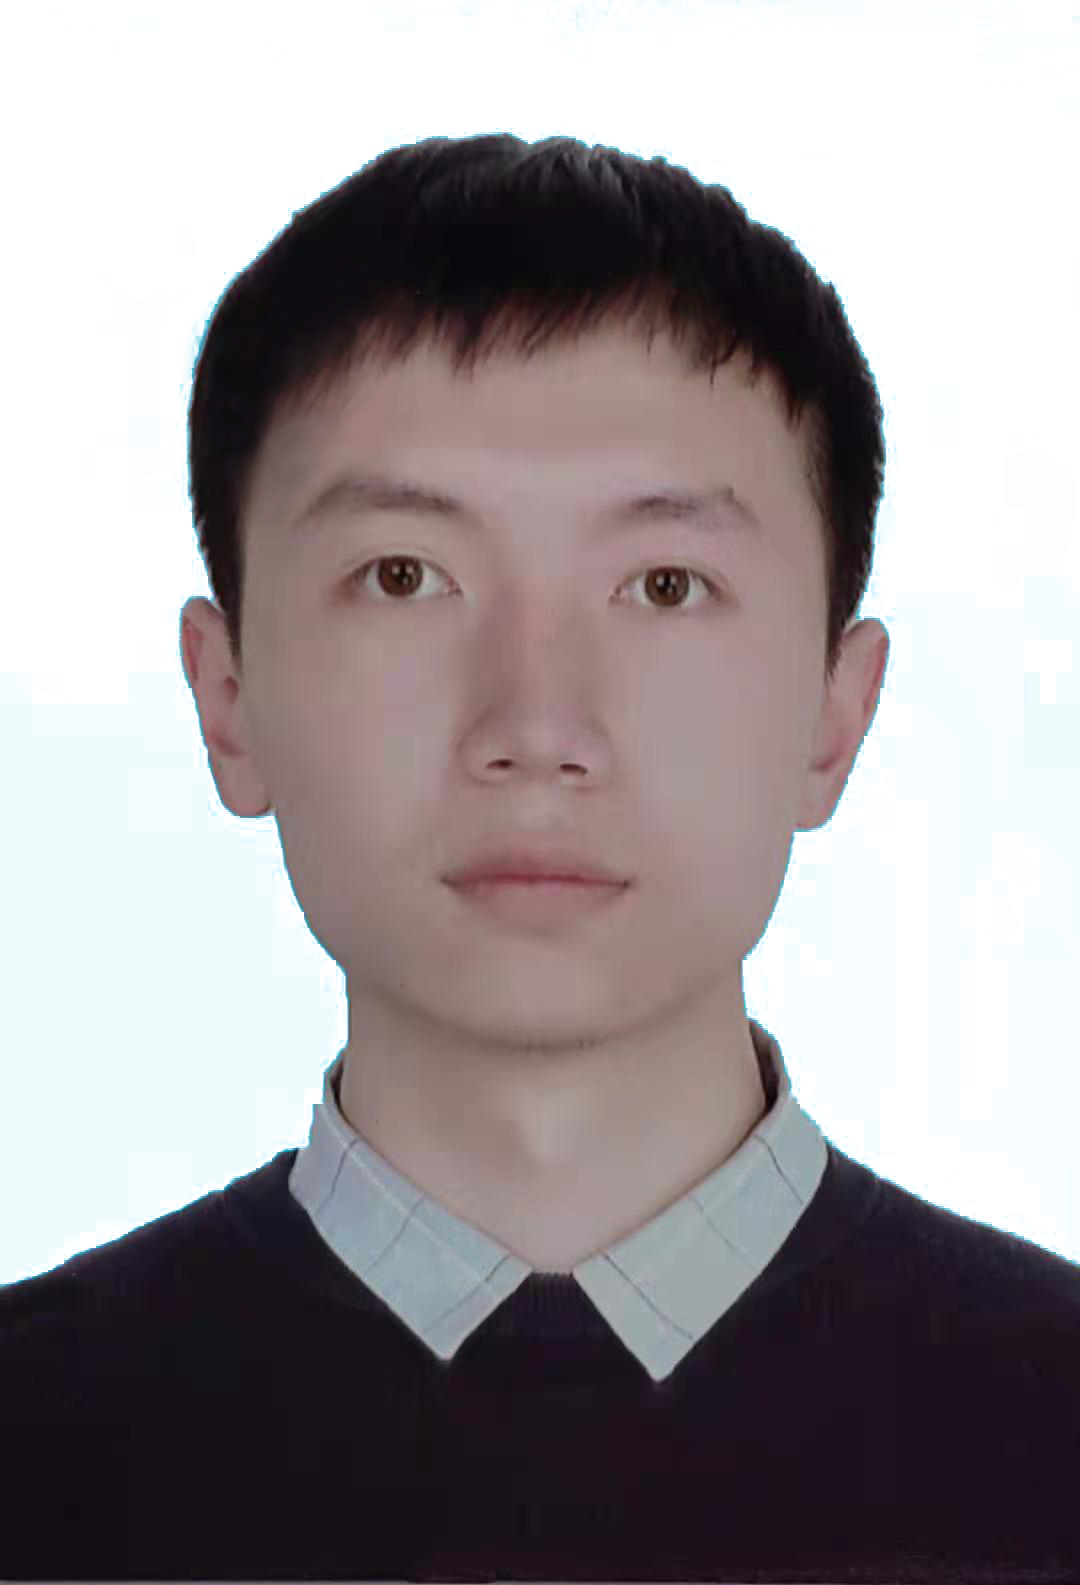
\includegraphics[width=1in,height=1.25in,clip,keepaspectratio]{./pic/author/zqh.jpg}}]{Qinghui Zhang}
	received a B.E. degree in software engineering from YangZhou University in 2020. He is currently working towards an M.S. degree at Yunnan University. His research interests include cloud computing and edge computing.
\end{IEEEbiography}



\begin{IEEEbiography}[{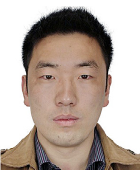
\includegraphics[width=1in,height=1.25in,clip,keepaspectratio]{./pic/author/lwd.png}}]{Weidong Li}
	received a Ph.D. degree from the Department of Mathematics of Yunnan University in 2010. He is currently a professor at Yunnan University. His main research interests are combinatorial optimization, approximation algorithms, randomized algorithms and cloud computing.
\end{IEEEbiography}

\begin{IEEEbiography}[{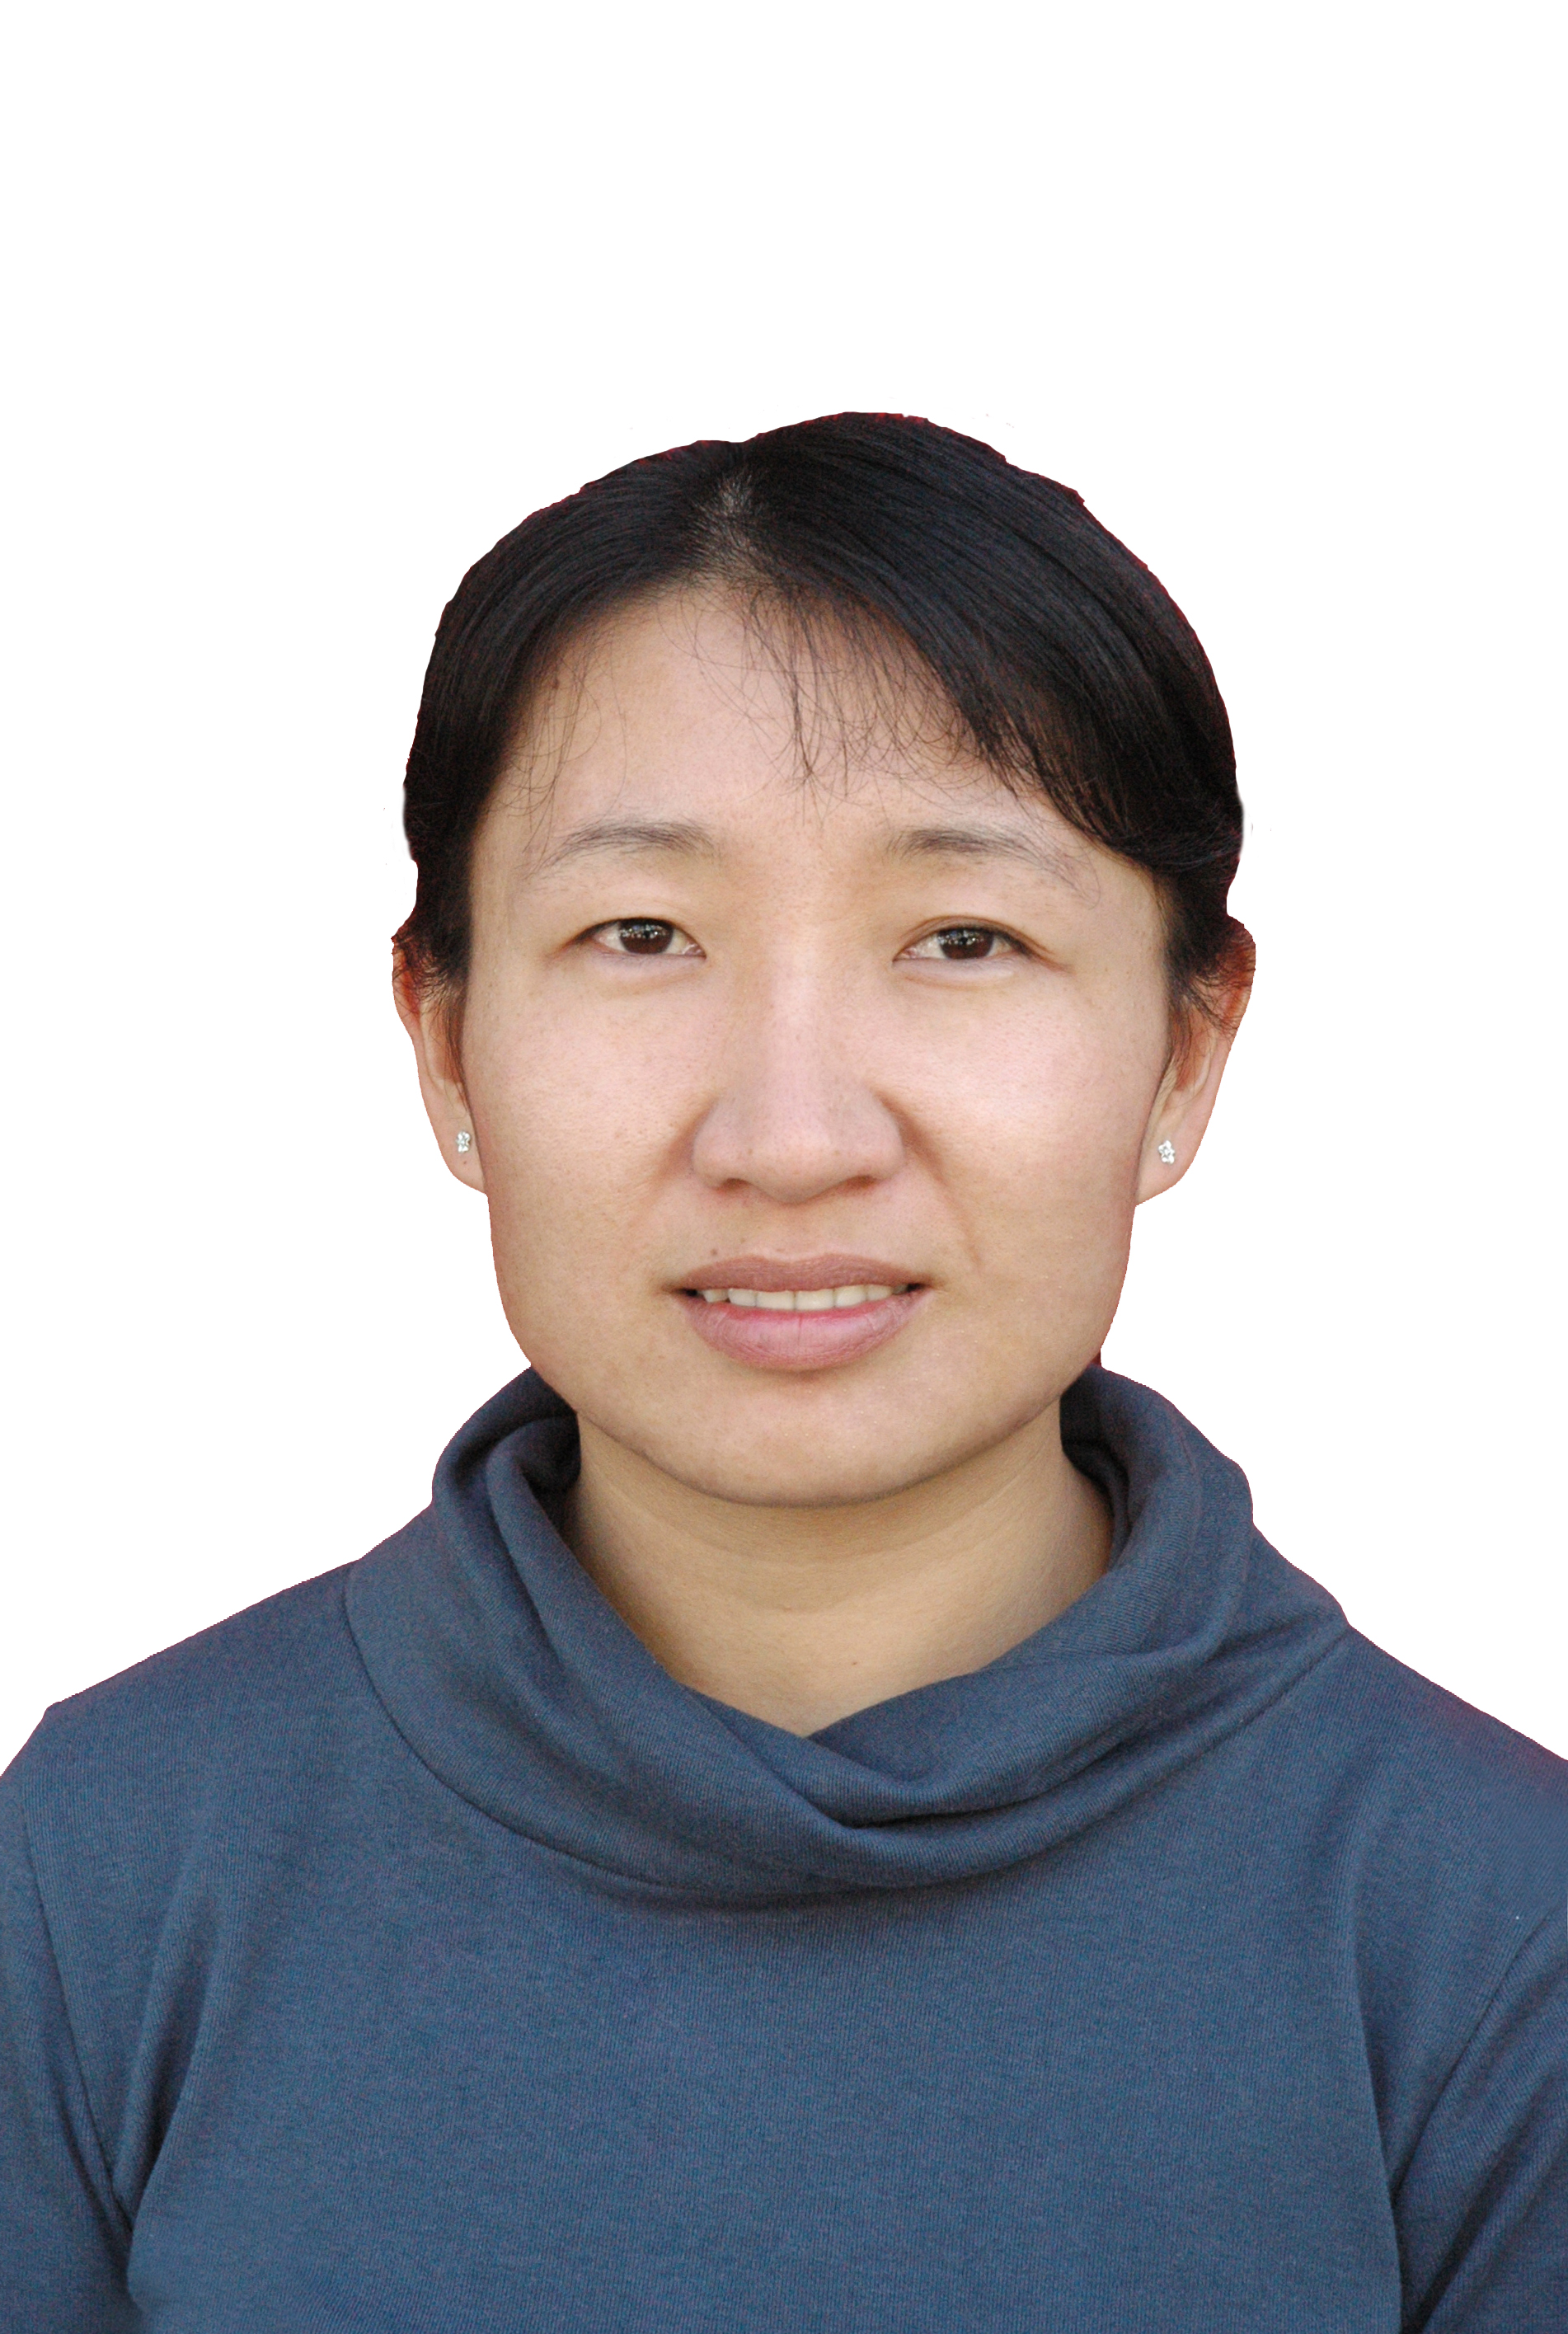
\includegraphics[width=1in,height=1.5in,keepaspectratio]{./pic/author/sq.jpg}}]{Qian Su}
	received a master's degree in computer
	science from Yunnan University in 2009. She is a lecturer and a Ph.D. candidate in the School
	of Information Science and Engineering, Yunnan University. Her research interests include edge
	computing and cloud-edge collaboration.
\end{IEEEbiography}



\begin{IEEEbiography}[{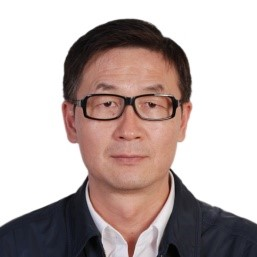
\includegraphics[width=1in,height=1.2in,keepaspectratio]{./pic/author/zxj.jpg}}]{Xuejie Zhang}
	received a master's degree in computer science and engineering from Harbin Institute of Technology in 1990. He received a Ph.D. degree in computer science and engineering from The Chinese University of Hong Kong in 1998. He is currently a professor in the Department of Computer Science and Engineering of Yunnan University. His main research interests are high-performance computing, distributed systems, computer networks and cloud computing.
\end{IEEEbiography}

% You can push biographies down or up by placing
% a \vfill before or after them. The appropriate
% use of \vfill depends on what kind of text is
% on the last page and whether or not the columns
% are being equalized.

%\vfill

% Can be used to pull up biographies so that the bottom of the last one
% is flush with the other column.
%\enlargethispage{-5in}



% that's all folks
\end{document}


